% ===================================================================
%  SoftwareX – Original Software Publication template (2025-05-13)
% ===================================================================
\documentclass[preprint,review,12pt]{elsarticle} % 'review' = line-numbers & wide margins
\journal{SoftwareX}

% ---------- packages you'll almost always need ----------
\usepackage{url}
\usepackage{hyperref}
\usepackage{graphicx}
\usepackage{amsmath,amssymb}
\usepackage{listings}      % nice code blocks
\usepackage{booktabs}      % classy tables
\usepackage{enumitem}      % compact lists


% ---------- front-matter ----------
\begin{document}
\begin{frontmatter}

\title{PowerPoint Accessibility Enhancer: An AI-powered Tool for Improving Presentation Accessibility}

\author[1]{Ibne Farabi Shihab\corref{c1}}
\ead{ishihab@iastate.edu}

\address[1]{Department of Computer Science,Iowa State University, Ames, USA}
\cortext[c1]{Corresponding author}

\begin{abstract}
The PowerPoint Accessibility Enhancer is a Streamlit-based web application designed to automatically improve the accessibility of PowerPoint presentations. It addresses critical accessibility issues including inadequate image descriptions, poor text readability, insufficient color contrast, and WCAG compliance gaps. Using AI-powered analysis and enhancement capabilities, the software enables content creators to make their presentations accessible to individuals with disabilities without requiring specialized knowledge. The tool combines local AI models with presentation processing libraries to provide a user-friendly interface for analyzing, fixing, and reporting on accessibility issues. PowerPoint Accessibility Enhancer is available as open-source software under the MIT license.
\end{abstract}

\begin{keyword}
accessibility \sep PowerPoint \sep WCAG \sep AI-powered enhancements \sep presentations \sep assistive technology
\end{keyword}
\end{frontmatter}

% ========================================================
%  1. Motivation and significance
% ========================================================
\section{Motivation and significance}
Accessibility is a crucial aspect of digital content creation that is often overlooked, particularly in educational and professional presentation materials. Despite the importance of accessible content for individuals with disabilities, many PowerPoint presentations lack proper accessibility features, making them difficult or impossible to use for people with visual, cognitive, or other impairments. According to the World Health Organization, approximately 15\% of the global population lives with some form of disability \cite{who}, and digital accessibility is increasingly recognized as a fundamental right.

Existing solutions to enhance presentation accessibility are limited, typically requiring manual implementation of accessibility best practices, which demands specialized knowledge and significant time investment \cite{accessibility-barriers}. Alternative solutions include using built-in accessibility checkers in software like Microsoft PowerPoint, but these tools only identify issues without providing automated fixes \cite{ms-accessibility}. 

The PowerPoint Accessibility Enhancer fills this critical gap by providing an automated solution that not only analyzes presentations for accessibility issues but also implements AI-powered fixes to enhance accessibility. This approach dramatically reduces the barrier to creating accessible content, allowing presenters to focus on their core message while ensuring their materials can be accessed by all audience members.

% ========================================================
%  2. Software description
% ========================================================
\section{Software description}
\subsection{Software architecture}
The PowerPoint Accessibility Enhancer follows a modular architecture designed for extensibility and maintainability, as illustrated in Fig. 1. The application consists of six primary components:

\begin{enumerate}
    \item \textbf{Frontend Module}: Built using Streamlit \cite{streamlit}, this component provides a web-based user interface that allows users to upload presentations, view analysis results, and apply accessibility enhancements.
    
    \item \textbf{Processing Engine}: Utilizes the python-pptx library \cite{python-pptx} to parse, analyze, and modify PowerPoint files. This module extracts content elements (text, images, shapes) and handles the serialization of modified presentations.
    
    \item \textbf{Analysis Module}: Evaluates presentations against WCAG (Web Content Accessibility Guidelines) \cite{wcag} standards, including text size, color contrast, alt text presence, and overall slide structure. It generates numerical accessibility scores for tracking improvements.
    
    \item \textbf{Enhancement Module}: Implements automated fixes for identified accessibility issues, including font size adjustments, color contrast improvements, and text simplification.
    
    \item \textbf{AI Integration}: Connects with Ollama \cite{ollama} running a LLaVA (Large Language and Vision Assistant) \cite{llava} model to provide AI-powered image understanding and description generation. This component includes service management to automatically start and configure required AI services.
    
    \item \textbf{Reporting Module}: Generates comprehensive accessibility reports detailing issues found, fixes applied, and remaining concerns in an exportable format.
\end{enumerate}

The project follows a modular code organization with separate components for core functionality such as accessibility checking, presentation analysis, enhancement processing, and the user interface.

This architecture enables the software to process presentations of varying complexity while maintaining good performance through optimizations such as parallelization of image processing, efficient memory management, and strategic caching of intermediate results.

\begin{figure}[h]
    \centering
    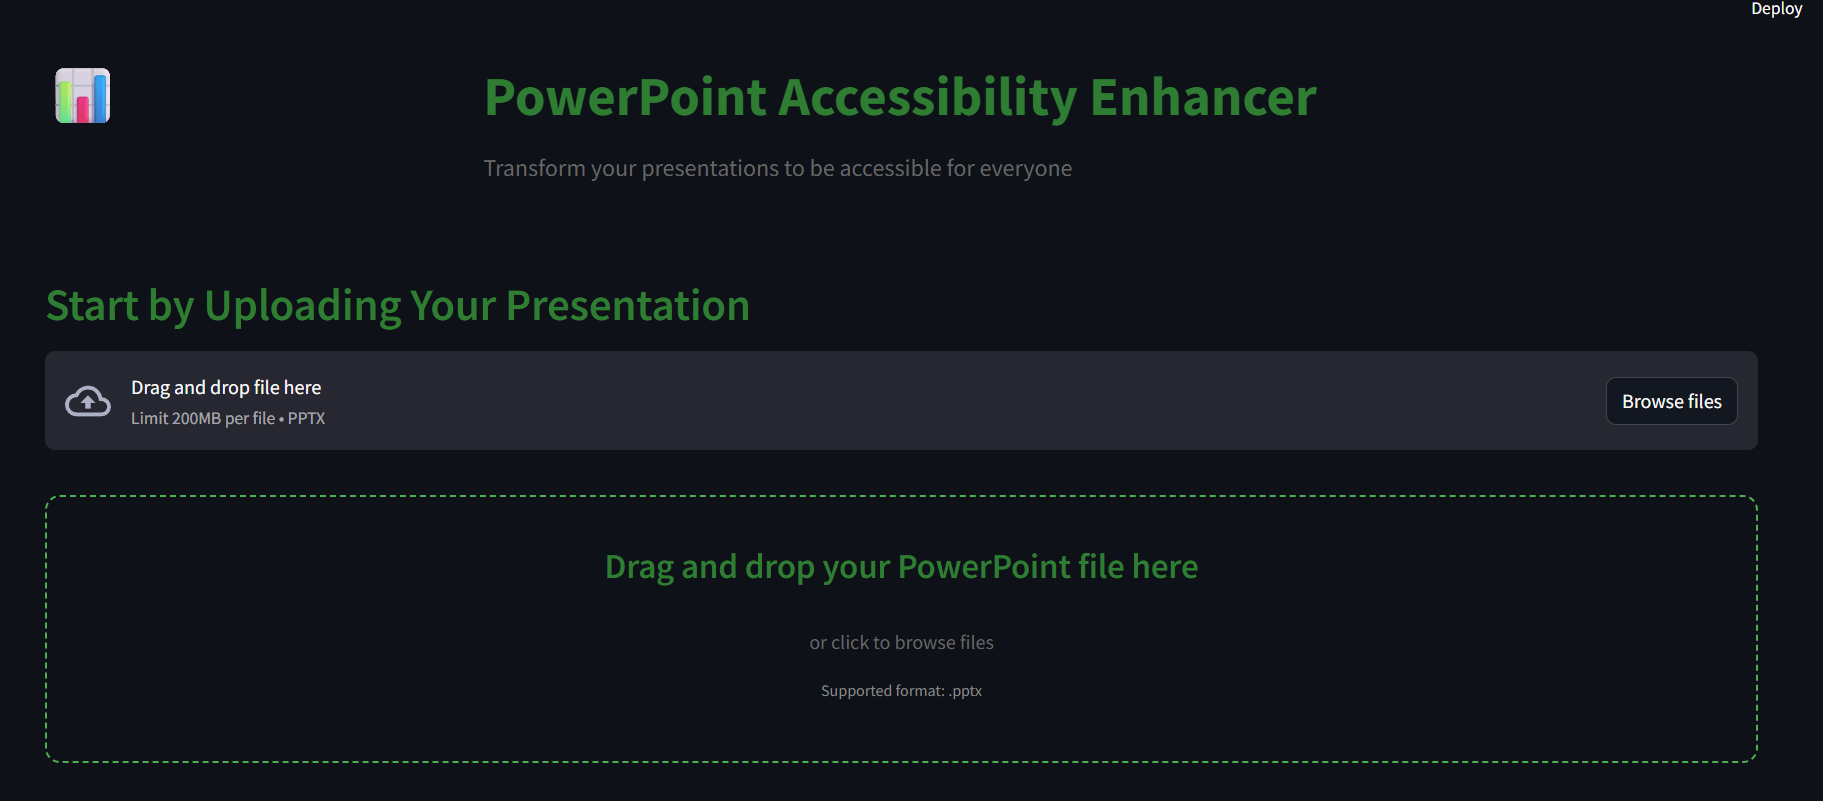
\includegraphics[width=\textwidth]{Figures/fig1_ppp.png}
    \caption{Initial interface of the PowerPoint Accessibility Enhancer showing the upload section where users can drag and drop or browse for their PowerPoint files. The clean, user-friendly interface makes the tool accessible to users without specialized knowledge in accessibility.}
    \label{fig:initial-interface}
\end{figure}

\subsection{Software functionality}
The PowerPoint Accessibility Enhancer provides comprehensive functionality for accessibility analysis and enhancement:

\begin{itemize}
    \item \textbf{Accessibility Analysis}: Evaluates presentations against WCAG \cite{wcag} standards, providing detailed reports on compliance issues including text size, color contrast, alt text presence, and slide structure.
    
    \item \textbf{AI-powered Alt Text Generation}: Automatically generates descriptive alternative text for images using the LLaVA \cite{llava} model, extracting images from slides and reintegrating context-aware descriptions. The system connects to a locally running LLaVA model via Ollama \cite{ollama}, which combines vision capabilities with language understanding to create contextually relevant image descriptions for screen readers.
    
    \item \textbf{Font Size Optimization}: Identifies and corrects text elements with insufficient size, automatically adjusting them to meet accessibility standards while preserving relative size relationships.
    
    \item \textbf{Color Contrast Enhancement}: Analyzes text-background color pairs for WCAG compliance (4.5:1 contrast ratio), automatically adjusting colors to improve readability while maintaining design aesthetics.
    
    \item \textbf{Text Simplification}: Evaluates text complexity using readability metrics and suggests or implements simplifications for overly complex language.
    
    \item \textbf{Comprehensive Reporting}: Generates detailed reports on accessibility issues found, changes made, and remaining concerns, with slide-by-slide analysis and severity ratings.
\end{itemize}

Figure \ref{fig:analysis-interface} shows the analysis interface where the software displays detailed accessibility metrics after analyzing a presentation.

\begin{figure}[h]
    \centering
    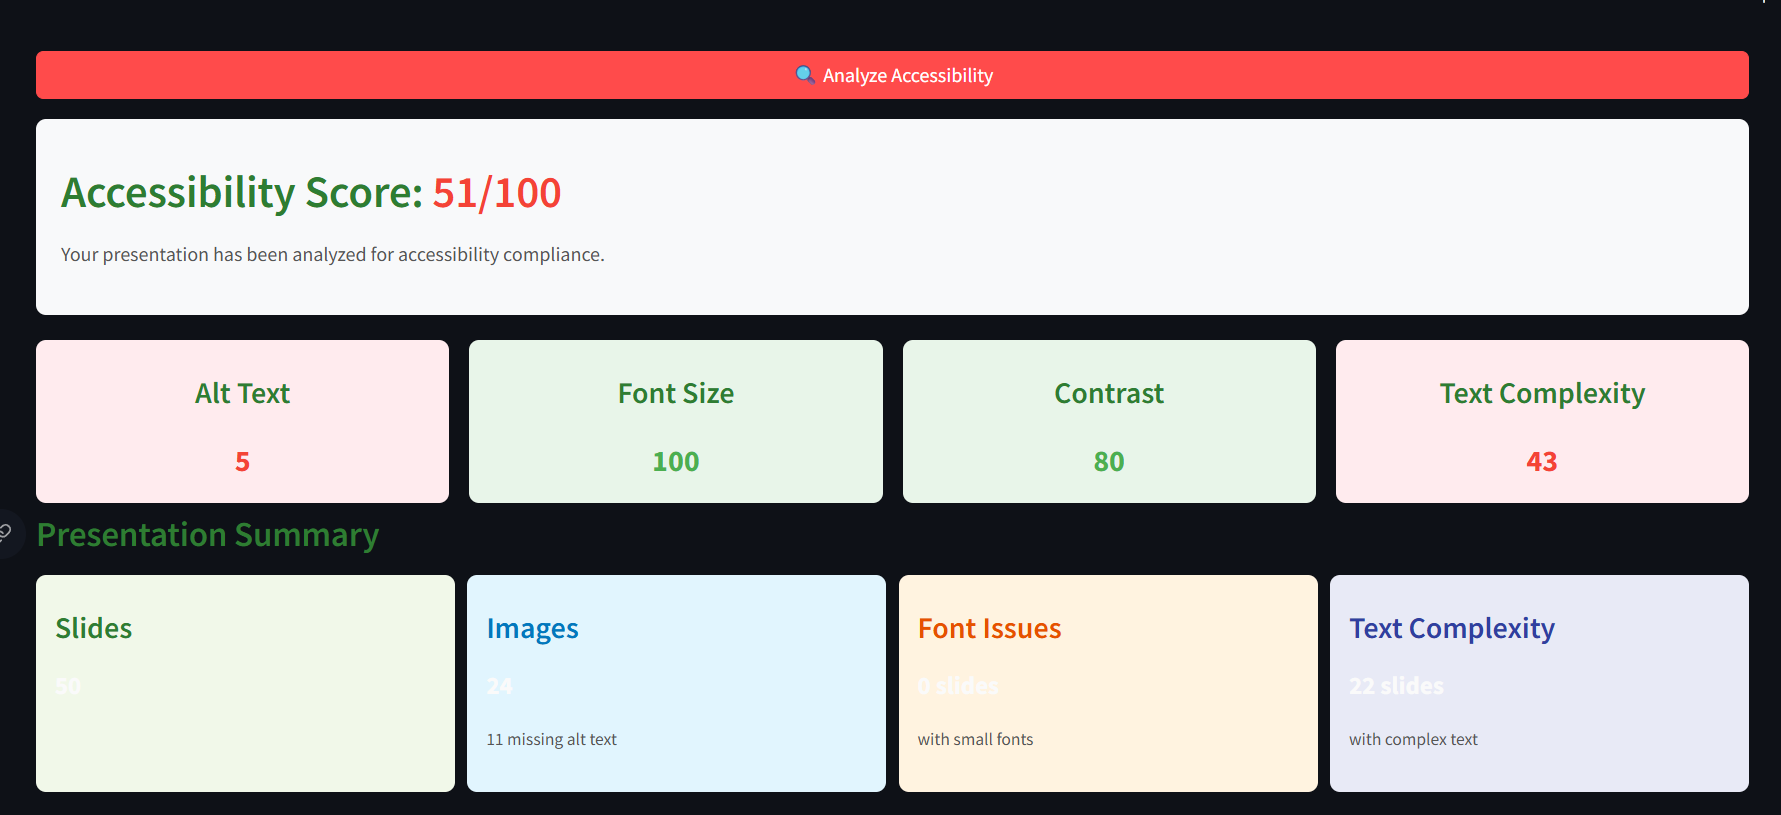
\includegraphics[width=\textwidth]{Figures/fig2_ppp.png}
    \caption{Analysis interface showing the accessibility evaluation results of a presentation. The system provides scores across multiple categories including alt text coverage, font size compliance, color contrast, and an overall accessibility score. Detailed findings help users understand specific accessibility issues that need to be addressed.}
    \label{fig:analysis-interface}
\end{figure}

A minimal example workflow involves uploading a PowerPoint file, reviewing the accessibility analysis, selecting enhancement options, and downloading the improved presentation file along with a detailed report.

\begin{lstlisting}[language=Python, caption=Example code for analyzing presentation accessibility]
# Import the PowerPoint Accessibility Enhancer
from ppt_accessibility import AccessibilityEnhancer

# Initialize the enhancer
enhancer = AccessibilityEnhancer()

# Analyze a presentation
analysis = enhancer.analyze_presentation("example.pptx")

# Generate and apply accessibility enhancements
enhanced_presentation = enhancer.enhance_presentation(
    "example.pptx",
    add_alt_text=True,
    fix_contrast=True,
    optimize_fonts=True,
    simplify_text=False
)

# Save the enhanced presentation
enhanced_presentation.save("example_enhanced.pptx")

# Generate an accessibility report
report = enhancer.generate_report()
report.save_html("accessibility_report.html")
\end{lstlisting}

After enhancement, users can download the improved presentation and view a detailed report of changes, as shown in Figure \ref{fig:result-interface}.

\begin{figure}[h]
    \centering
    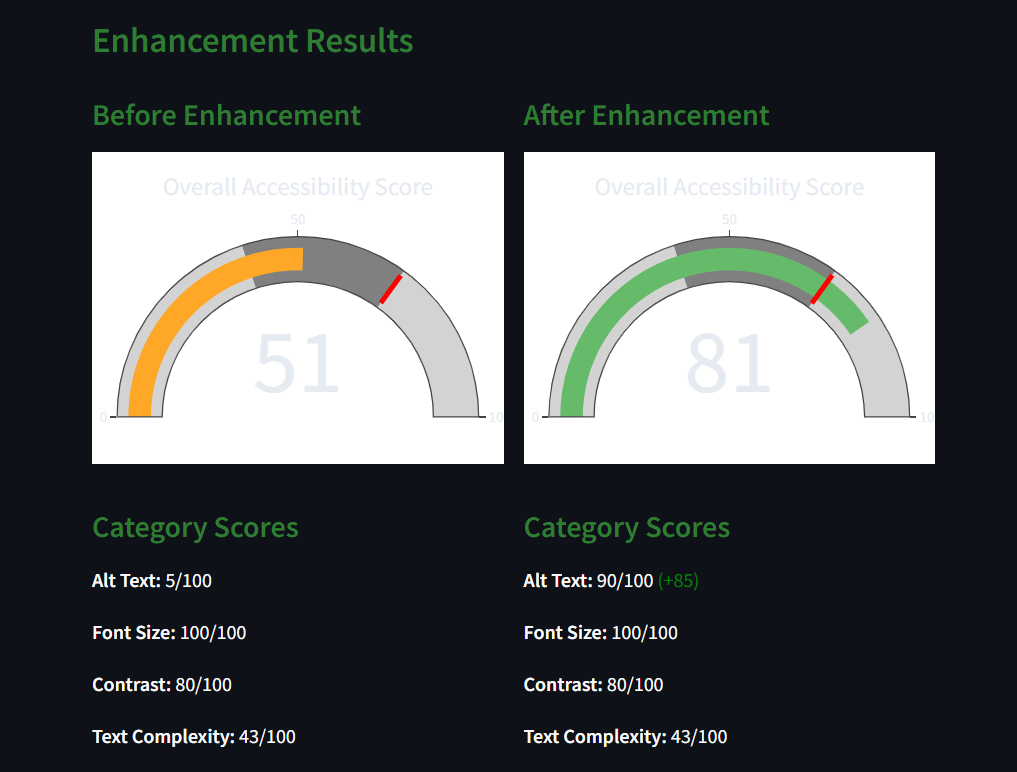
\includegraphics[width=\textwidth]{Figures/fig3_ppp.png}
    \caption{Results interface showing the enhanced presentation with accessibility improvements applied. The interface displays the before and after accessibility scores, highlighting the improvements made. Users can download both the enhanced presentation and a detailed HTML report documenting all accessibility changes.}
    \label{fig:result-interface}
\end{figure}

\subsection{Installation and usage}
The PowerPoint Accessibility Enhancer is designed for ease of installation and use across multiple platforms (Windows, macOS, and Linux). Installation involves three main steps:

\begin{enumerate}
    \item Cloning the repository
    \item Installing Python dependencies via pip
    \item Installing and configuring Ollama with the LLaVA model for AI-powered alt text generation
\end{enumerate}

The application includes platform-specific launchers (launcher.bat for Windows and launcher.sh for Linux/Mac) that automate the process of starting both the Ollama service and the Streamlit application. For users preferring manual control, the application can be started by running the Ollama service separately and then launching the Streamlit application.

\begin{lstlisting}[language=bash, caption=Manual startup process]
# Start Ollama with the LLaVA model
ollama run llava

# In a separate terminal, run the Streamlit app
streamlit run app.py
\end{lstlisting}

Once running, users interact with the application through a web browser interface at http://localhost:8501, where they can upload presentations, analyze accessibility issues, apply enhancements, and download the improved files.

The application also includes fallback mechanisms when Ollama is not available, using basic placeholder text for image descriptions to ensure the software remains functional even without the AI capabilities.

\subsection{Limitations and technical considerations}
The PowerPoint Accessibility Enhancer has several known limitations:

\begin{itemize}
    \item \textbf{WMF/EMF Images}: Windows Metafile (WMF) and Enhanced Metafile (EMF) images cannot be processed by the AI for alt text generation due to format incompatibility. These images receive generic descriptions instead.
    
    \item \textbf{Complex Layouts}: Very complex slide layouts with overlapping elements or unusual positioning may not be perfectly analyzed for reading order or structure.
    
    \item \textbf{Font Embedding}: Some custom fonts used in presentations may not be properly detected for size analysis if they are not embedded correctly.
    
    \item \textbf{Network Requirements}: The application relies on local network connectivity between the Streamlit application and the Ollama service (typically on port 11434), which may require special configuration in restricted network environments.
\end{itemize}

These limitations are documented in the application's troubleshooting guide, along with potential workarounds and solutions where available.

% ========================================================
%  3. Impact
% ========================================================
\section{Impact}
The PowerPoint Accessibility Enhancer has significant potential impact across multiple domains where presentations are regularly used for communication and education:

\textbf{Educational Impact}: In educational settings, accessible presentations ensure that learning materials are available to all students, regardless of disabilities. Educators who may lack accessibility expertise can now easily create inclusive materials, supporting principles of universal design for learning \cite{udl}.

\textbf{Professional Environment}: Organizations facing legal requirements to provide accessible content (such as those under Section 508 in the US or the European Accessibility Act) can use this tool to efficiently achieve compliance without extensive training or resources \cite{section508}.

\textbf{Accessibility Research}: The tool provides a platform for researching and implementing new approaches to automated accessibility enhancement, potentially extending beyond presentations to other document formats.

\textbf{Disability Inclusion}: By removing barriers in presentation materials, the software promotes fuller participation of individuals with disabilities in educational, professional, and social contexts where presentations are used.

Early adopters include educational institutions seeking to improve the accessibility of teaching materials, corporate training departments aiming to ensure compliance with accessibility regulations, and individual content creators committed to inclusive design principles. Feedback from these users has highlighted significant time savings compared to manual accessibility improvements and increased confidence in meeting accessibility standards.

The modular architecture and open-source nature of the software enable researchers and developers to extend its capabilities to additional document types and accessibility criteria, potentially broadening its impact across digital content creation.

% ========================================================
%  4. Conclusion
% ========================================================
\section{Conclusion}
The PowerPoint Accessibility Enhancer represents a significant advancement in automated accessibility tools, combining AI capabilities with accessibility expertise to enable non-technical users to create more inclusive content. By addressing key barriers to presentation accessibility including image descriptions, text readability, and color contrast, the software helps content creators reach wider audiences and comply with accessibility standards.

Future development will focus on extending support to additional presentation formats (Google Slides, Keynote), implementing advanced layout optimization for screen readers, integrating with additional AI models, adding batch processing capabilities, and developing API endpoints for integration with other systems. These enhancements will further reduce barriers to creating accessible content across platforms.

The project demonstrates how AI technologies can be leveraged to solve real-world accessibility challenges, potentially serving as a model for similar tools in other content domains. As accessibility regulations continue to evolve globally, tools like the PowerPoint Accessibility Enhancer will play an increasingly important role in enabling compliance and promoting inclusive digital experiences.

% ========================================================
%  Required OSP tables
% ========================================================
\section*{Code metadata}
\begin{table}[h!]
\small
\centering
\begin{tabular}{@{}ll@{}}
\toprule
\textbf{Nr.} & \textbf{Description} \\ \midrule
C1 & Current code version: \texttt{v1.0.0} \\
C2 & Permanent link to code/repository: \url{https://github.com/farabi1038/powerpoint_asccessibility_project} \\
C3 & Legal Code Licence: MIT Licence \\
C4 & Code versioning system used: \texttt{git} \\
C5 & Software languages, tools, services: Python, Streamlit, Ollama, PIL/Pillow \\
C6 & Compilation requirements, dependencies: Python $\geq$3.10, python-pptx, Streamlit $\geq$1.22.0, Ollama $\geq$0.1.2, LLaVA model \\
C7 & Link to developer documentation/manual: \url{https://github.com/farabi1038/powerpoint_asccessibility_project/blob/main/README.md} \\
\bottomrule
\end{tabular}
\end{table}

\vspace{1em}
\noindent\textbf{CRediT authorship contribution statement}\\
\textbf{Ibne Farabi Shihab}: Conceptualization, Methodology, Software, Writing -- original draft.

\vspace{0.5em}


% ========================================================
%  References
% ========================================================
\bibliographystyle{elsarticle-num}
\bibliography{references}   % your BibTeX file

\end{document}
